\section{Evaluation}
\label{sec:results}

We evaluate three claims: direct estimation avoids shrinking-target noise; local scores support useful cavity placement; and sparse queries can reduce computational cost relative to a global discretized solve. Matched pipelines on a finned housing, branching manifold, and annular spreader test placement and numerical cost under shared constraints. The Bunny supplies a detailed-geometry stress test and a count--radius study, while controlled experiments isolate statistical effects. Earlier thermal studies retain their original protocols and are summarized separately. \Cref{app:experiments,sec:critical} retain full protocols, secondary plots, solver checks, and all measured comparisons.

\paragraph{Common physics and decision rule.}
All 3D design studies solve $-\Delta u=f$ with nonnegative internal heating and ideal zero-temperature exterior and cavity walls. The sensor-protection pipelines and accessible-channel studies minimize the regional objective $J_q=\int qu/\int q$ with a distinct adjoint; the compact sensor weight in the new matched study is normalized to integrate to one. The earlier Bunny, housing-compliance, and guarded-validation studies minimize compliance $J=\int fu$ under prescribed removal and clearance constraints. Their relative reductions use a fixed original-domain normalization and fresh objective samples. For compliance, $p=u$ and the candidate benefit is $u^2$; a cross-fitted score uses distinct walk indices even when the same samples represent both fields. Each insertion changes the domain before the next score evaluation. The ranking studies use fresh shortlist samples. \Cref{sec:applicationvalidation} separately evaluates a guarded compliance selector.

\paragraph{Measured comparisons.}
The deterministic design baselines use a voxel adjoint field with either conjugate gradients or geometric multigrid; they evaluate the same topological score and share the candidate and cavity budgets. Random feasible placement tests whether the score helps beyond adding cold surface. Same-seed multiplication and finite-cavity differencing isolate estimator choices. Array-RQMC and neighbor reuse are studied separately as compatible accelerations. The external FEM experiment checks initial fields, and the probabilistic-shape and spectral-connectivity experiments check components; none is presented as a reproduced full external optimizer.

\subsection{Matched design pipelines on distinct geometry}
\label{sec:submissionstudy}

We next isolate three questions that a cavity-count comparison alone cannot
answer: whether objective-aware nucleation improves subsequent boundary
optimization; whether accessible-channel improvements survive fixed material
and power budgets; and whether the shrinking-target comparison transfers to
actual three-dimensional application meshes. The finned housing, branching
manifold, and ribbed annular spreader in \cref{fig:submissiongeometries} have
narrow gaps, branching paths, or curved transport and a thin central bridge.
Their protected sensors and complete compact heat-source supports remain
unchanged under every design. \Cref{app:submissionstudy} specifies the physics,
normalizations, geometry constraints, and numerical checks.



\paragraph{Nucleation followed by Differential WoS.}
All methods place six disjoint spheres of radius $0.065$ from the same paired
candidate pools, then optimize their centers using a common specialized
implementation of Differential WoS~\cite{miller2024differential}.
TWoS and deterministic topological derivatives use eight refinement rounds;
hottest-point and random initializations also receive rounds nine through
sixteen. Two complete deterministic baselines use longest-axis grid counts
49 and 65. A nearest-sensor control replaces the PDE score by Euclidean
distance to the protected sensor and receives eight refinement rounds. The curves in \cref{fig:submissionpipeline} report complete design
costs at independently evaluated checkpoints. This comparison isolates the
value of initialization inside a shared optimizer; it does not compare against
the original authors' full application or assert that Differential WoS cannot
change topology.

Across five paired seeds, TWoS followed by eight refinement rounds yields
mean sensor reductions of $65.0\%$, $16.4\%$, and $11.4\%$ on the housing,
branching manifold, and annular spreader. The primary multigrid selector followed
by the same refinement yields $65.1\%$, $16.3\%$, and $11.7\%$.
Hottest-point initialization with sixteen rounds yields $42.7\%$, $0.14\%$,
and $0.01\%$, respectively. Both TD selectors perform similarly in these
comparisons; their numerical costs and the additional controls are reported
in the full time--quality curves and \cref{tab:submissionpipeline}.
The nearest-sensor control yields $63.6\%$, $17.3\%$, and $12.2\%$
across the same three objects. On the housing it requires $7.08$ s, compared
with $11.77$ s for TWoS.
Thus the large contrast with hottest-point placement does not establish a
large benefit over every informed heuristic. The cutaways show this stronger
geometric control alongside TWoS and multigrid; the plots retain all methods.
The bands describe uncertainty in measured mean cooling, not equivalence tests
or guarantees for a new geometry.


\paragraph{Accessible channels at matched volume and fixed power.}
Six parallel open ball-union channels target total removed volume $0.0168$.
Their common radius is recalibrated after each insertion, and independent
scrambled-Sobol samples audit the final volume. All heat supports are protected,
so their exact input power is invariant (\cref{prop:protectedpower}).
\Cref{fig:submissionchannels} reports these finite designs. A pointwise
axis score initializes the channels; it is not a topological derivative of
an entire channel, and the radius calibration is numerical rather than certified.
At this matched budget, TWoS yields mean reductions of $37.8\%$, $2.29\%$,
and $1.75\%$ across the three objects, compared with $42.1\%$, $2.59\%$,
and $1.93\%$ for the primary multigrid selector. On the housing, nearest-sensor
placement yields $39.4\%$, and the cheaper multigrid grid attains the same
mean reduction as the primary grid. Thus this finite-channel heuristic does
not dominate the informed controls. \Cref{tab:submissionchannels} reports all
methods and uncertainty intervals; the independent volume and reference audits
remain separate from those sampling intervals.

\paragraph{Variance, bias, and query cost.}
\Cref{fig:submissionestimators} compares direct scores, common-random-number
finite-cavity subtraction, a stronger stopped-path harmonic-correction
baseline, and multigrid at four resolutions on eight fixed sites per object.
Sixteen independent repeats resolve sampling variability. Relative variance
about each method's mean is shown separately from error to a high-budget
infinitesimal reference: finite-cavity methods retain finite-radius bias,
while multigrid retains discretization error. The reference itself has
sampling and termination error. Bands around variance describe uncertainty
in the estimated variance, not a standard-deviation envelope of field values.
\Cref{app:submissionstudy} gives the stronger finite-correction identity and
its step-by-step proof; detailed numeric summaries accompany the source.
At radius $0.01$ and 2,048 paths per site, the stronger harmonic-correction
baseline has $35.7\times$ and $13.8\times$ the measured direct variance on
the housing and branching object. These are point estimates, not confidence
bounds. On the annular object, all recorded harmonic corrections vanish at
radii $0.01$ and $0.02$; variance is unresolved, and collapsed bootstrap
intervals are suppressed. At larger radii the stronger correction can have
competitive measured variance. Direct TWoS relative RMS error at this budget
is $14.9\%$, $25.2\%$, and $146\%$ across the three cases, while the
reference's relative standard-error norms are $1.6\%$, $4.8\%$, and
$16.2\%$. The annular sparse-query configuration is poorly resolved at these
budgets; it is not evidence of uniformly accurate pointwise estimation.

The maximum independent channel-volume audit deviation is $0.97\%$ of the
target. Finer housing checks change by at most $0.44$ percentage points from
grid 193 to 257, but MC--grid257 differences still reach $2.38$ points across
the checked first-seed states. Sampling intervals do not absorb this numerical
reference sensitivity (\cref{tab:submissionfinereference}).


\subsection{Protecting a region with a distinct adjoint}
\label{sec:regional}

Compliance makes the adjoint equal to the state. To test whether
objective-aware scoring matters beyond finding hot spots, we keep the
housing's heat sources fixed and minimize the weighted mean temperature
of a protected sensor region. The objective is
$J_q=\int q u/\int q$, where $q$ is a compact nonnegative bump in
a radius-$0.13$ ball. The adjoint solves $-\Delta p=q$, and candidates
are ranked by $up$. This differs from the hottest-point score $u$.
Two sensor placements test the left and right sides of the same housing;
they are two objectives, not two independent input geometries.
All cavities must avoid the sensor region with an additional $0.02$
gap, so no design can improve the objective by deleting the sensor.
\Cref{app:regional} derives the normalization, adjoint, and an exact
counterexample to hottest-point placement.

Each of five paired candidate/design seeds supplies 768 candidates.
Every method places six radius-$0.095$ cavities under the same clearance
constraints. We compare sparse \method{} (12 scouting and 192 rescoring
walks), a larger budget (48 and 768), WoS hottest-point placement at the
sparse budget, deterministic multigrid hottest-point placement,
multigrid topological derivatives, and random feasible placement.
The 24-site rescore uses fresh walks. Paired state--adjoint queries
share paths within each pair and use the cross-index product.
Multigrid reuses one geometry hierarchy for its two right-hand sides.
The primary grid is $113\times73\times57$; a supplementary sweep
adds $57\times37\times29$, $85\times55\times43$, and
$169\times109\times85$ without discarding unfavorable results.

Sparse \method{} reduces the left/right regional objectives by $50.87\%$ /\allowbreak $50.09\%$, compared with $38.15\%$ /\allowbreak $29.99\%$ for deterministic hottest-point placement. The primary multigrid topological selector gives $53.30\%$ /\allowbreak $52.15\%$. Averaged across both cases, complete sparse \method{} design takes $3.66$\,s, versus $8.38$\,s for the primary multigrid setting. The fastest tested multigrid setting (57 nodes along the first axis) takes $2.51$\,s and gives $53.50\%$ /\allowbreak $52.53\%$ reduction. Retaining the outer mesh in one process per complete adaptive design reduces wall time to $1.22$\,s for sparse \method{}, $1.41$\,s for coarse multigrid, and $7.13$\,s for primary multigrid. All 70 repeated designs have exactly the same six sequential cavity centers as their original runs, permitting reuse of the independent objective evaluations. These results demonstrate an advantage over hottest-point placement; the full budget sweep in \cref{fig:regional,tab:regional} qualifies comparisons with volumetric topological derivatives.


Complete design wall times include common candidate preparation,
geometry setup, source queries or PDE solves, candidate filtering,
ranking, subprocess startup, and file I/O. The retained-mesh backend
keeps the fixed outer boundary acceleration structure alive throughout
each six-round design, for both Monte Carlo and multigrid methods.
Candidate filtering, fresh rescoring, and every adaptive insertion still
execute inside the measured driver; future requests are not replayed
ahead of those decisions. Offline reference evaluation
is measured separately. Both a fresh WoS evaluation and a separate
$169\times109\times85$ multigrid solution assess every final design.
These are approximate references; first-seed designs additionally
receive a fourfold WoS shell refinement and a $225\times145\times113$
grid check. The designs use fixed-count ranking, not the
compliance-only finite-benefit certificate. The comparison against
hottest-point placement tests the adjoint's value, which is shared
with deterministic topological derivatives; the quality--cost
comparison tests the choice of numerical estimator.



\subsection{Accessible channels and protected components}
\label{sec:accessible}
We next replace sealed cavities with vertical through-channels in the
housing. Every channel is a union of 18 radius-$0.075$ balls, spanning
both exterior sides. Their spacing gives a guaranteed continuous
passage of radius $0.075\sqrt{3}/2$; \cref{app:accessible} proves this
geometric statement and the component-clearance predicates. The
sensor and three prescribed component regions cannot be removed.
Port positions vary with the selected axes. We retain the ideal cold-wall
model, so geometric access does not establish coolant delivery or
realistic heat transfer.

This is an application of point scoring to a larger geometric operation:
the algorithm scores candidate axes at a common interior plane and
inserts the complete channel. The pointwise topological coefficient
is a placement proxy here, not a derived whole-channel derivative.
All five methods use the same candidate axes, six-channel count,
radius, extent, and protection constraints. We repeat both sensor
objectives over five paired seeds and evaluate all 50 completed
designs independently. Removed volume is reported because local
housing thickness varies; this is not an equal-volume experiment.

On the left and right sensors, the TWoS proxy gives reductions of $55.74\%$ and $52.47\%$, versus $43.78\%$ and $30.39\%$ for hottest-point placement. Mean complete design times are $1.02$\,s for TWoS and $1.26$\,s for coarse multigrid. Their mean reductions across both sensors are $54.10\%$ and $57.55\%$, respectively. This preserves a useful quality--cost tradeoff under access constraints, without establishing superiority over deterministic topological scoring.





\subsection{Thermal design on a finned housing}

A closed 96,740-triangle procedural housing contains three localized Gaussian heat sources. Each method places six radius-$0.095$ cavities from 768 shared Sobol candidates. Sparse \method{} uses 12 scouting walks per feasible site and 192 fresh walks on a 24-site shortlist; a larger budget uses 96 and 768 walks. A predeclared field-error criterion selects the multigrid grid, $113\times73\times57$, from a resolution sweep. Both algorithms run in the same C++ executable. Selection time includes geometry acceleration and all six rounds of querying or global solving; it excludes file I/O, process startup, and the common independent objective evaluation.



Across five complete stochastic design seeds, sparse \method{} reduces compliance by $68.90\%\pm0.84\%$ (standard error), compared with $70.36\%\pm0.08\%$ for the deterministic multigrid design, whose uncertainty comes from objective evaluation. Mean selection time is $0.432$ s versus $1.861$ s: $4.31\times$ faster while achieving $97.9\%$ of the measured reduction. The larger \method{} budget gives $69.39\%\pm0.51\%$ reduction in $1.731$ s, using $19.1$ MiB peak RSS versus $31.4$ MiB. Random placement gives $27.76\%\pm4.57\%$. These are quality--cost tradeoffs over the tested designs; the seed count does not establish equivalence or superiority in design quality. The multigrid sweep and resource curves appear in \cref{fig:housingtradeoffs}. This earlier compliance comparison uses a field-error-selected grid and excludes driver costs; the regional pipelines in \cref{sec:submissionstudy} include those costs and both cheaper grids. Its speed ratio should not be transferred between these protocols.

An independent scikit-fem implementation on 393,616 tetrahedra checks the initial ranking. The 512-walk field has Pearson correlation $0.9943$ and $95\%$ top-20 overlap with that FEM field. Its boundary approximation and convergence are documented in \cref{fig:externalaudit}; the FEM audit is an accuracy comparison, not an optimized FEM timing baseline.

\subsection{Detailed geometry and sparse-query scaling}

We repair and close the Stanford Bunny~\cite{stanford1994bunny}, obtaining 69,674 triangles, and normalize its height to one. With affine heating $f(x,y,z)=1+0.65(y+0.5)$, each method places six radius-$0.05$ cavities among 1,024 candidates. \method{} uses a 12-walk scout and fresh 128-walk rescoring of 20 sites. Its measured compliance reduction is $47.77\%$, compared with $48.06\%$ for the $54\times64\times48$ voxel adjoint and $39.46\%$ for random placement. This single-run test demonstrates placement on detailed geometry; the replicated allocation study below supplies a broader design comparison.

A separate matched C++ experiment isolates query cost on the original Bunny. At 64 requested sites, 512-walk \method{} takes $0.381$ s and $15.4$ MiB peak RSS; voxel FD/CG takes $0.528$ s and $80.7$ MiB. The corresponding relative score errors against an independent 16,384-walk reference are $5.89\%$ and $6.89\%$. This is $1.39\times$ faster evaluation with $81\%$ less peak memory, at similar measured error. The numerical reference itself has sampling and termination error. The methods tie near 96 sites, and at 384 sites the voxel solve is faster ($0.504$ s versus $2.10$ s). \Cref{fig:compiledbunny} reports the full sweep. These timings establish a sparse-query advantage, not a speedup for the displayed Bunny optimization.



\subsection{Cavity count at fixed removed volume}
\label{sec:bunnybudget}

Does cooling improve because placement is better, or simply because more
material is removed? We separate these effects with 72 Bunny designs:
two exact volume budgets, four counts $n\in\{2,4,6,12\}$, three independent
design seeds, and \method{}, voxel-adjoint TD, and random feasible placement.
The budgets equal three or six radius-$0.05$ balls: $0.765\%$ or $1.529\%$
of the original Bunny volume. Within each allocation, every cavity has
radius $r_n=0.05(b/n)^{1/3}$, where $b\in\{3,6\}$ is the budget in ball-volume
units. Radii follow this constraint; only centers are optimized. All methods
share 1,024 candidates within each seed/allocation, retain outer clearance
$0.012$ and pairwise surface gap $0.014$, and start from the unperforated domain.
TWoS retains the 12-walk scout and independent 128-walk shortlist rescoring;
this ranking heuristic is not a finite-insertion confidence certificate.
The compiled voxel selector uses a finer $96\times112\times84$ FD/CG grid
than the original Bunny design test.



% The following measured paragraph is populated from the retained summaries.
At the full volume budget, increasing the TWoS count from two to twelve raises mean cooling from $37.58\%$ to $54.33\%$, while the radius decreases from $0.0721$ to $0.0397$. At twelve cavities, the voxel and random means are $55.02\%$ and $38.78\%$, respectively. The most useful allocation comparison is across budgets: twelve small TWoS cavities at half volume yield $47.26\%$ cooling (design range $47.03$--$47.67\%$), versus $47.45\%$ ($46.78$--$48.22\%$) for six larger cavities at full volume. The former also has $20.6\%$ less cavity surface area, by exact sphere geometry. This is similar measured cooling with less removal, not a proved equivalence or an advantage unique to TWoS. The voxel selector shows a similar allocation trend. A fourfold thinner WoS termination shell, $1.25\times10^{-4}$, changes cooling by at most $0.204$ percentage points for the pre-specified first-seed full-budget endpoint designs from both TD selectors. This sensitivity check does not bound the remaining bias.
An additional first-seed check of the half-volume comparison, chosen after inspecting the allocation results, gives $46.88\%$ versus $47.21\%$ cooling with the thinner shell, respectively.


All objective comparisons use four independently scrambled 512-point
interior blocks and 128 WoS paths per active point, separate from selection.
Removed material contributes zero under fixed original-volume normalization;
reported percentages average paired block ratios to the initial state.
Design ranges and conditional block standard errors are retained separately;
three seeds do not establish equivalence or a globally optimal allocation.

\paragraph{Why a preferred count needs a cost.}
Additional nested ideal cooled removal lowers compliance exactly
(\cref{prop:coolingmonotonicity}), whereas different equal-volume allocations
are not nested. At fixed removed volume $V$, exposed area grows as $n^{1/3}$
and the sum of isolated capacities as $n^{2/3}$ (\cref{prop:budgetgeometry});
the latter is not the interacting union capacity. A volume-only penalty is
constant within this sweep. Instead, \cref{fig:bunnybudget}c illustrates
$J/J_0+\kappa n$ for an explicitly assumed count cost. This isolates the
modeling choice behind a ``sweet spot'' without attributing it to the
topological estimator or claiming an application-specific optimum.


\subsection{Estimator accuracy and sampling uncertainty}

The annulus diagnostic has an exact capacity and cavity-hit probability, making the rare-event comparison analytically controlled. With 256 samples per estimate and 3,000 repetitions, fitted variance slopes versus capacity are $0.00$ for direct estimation, $-1.10$ for coupled differencing, and $-1.89$ for independent differencing. At the smallest tested capacity, direct variance is $8.26\times$ lower than the coupled baseline. This experiment tests the shrinking-target mechanism under its stated model; it does not rule out importance samplers conditioned on cavity hits.

\begin{figure}[t]
 \centering
 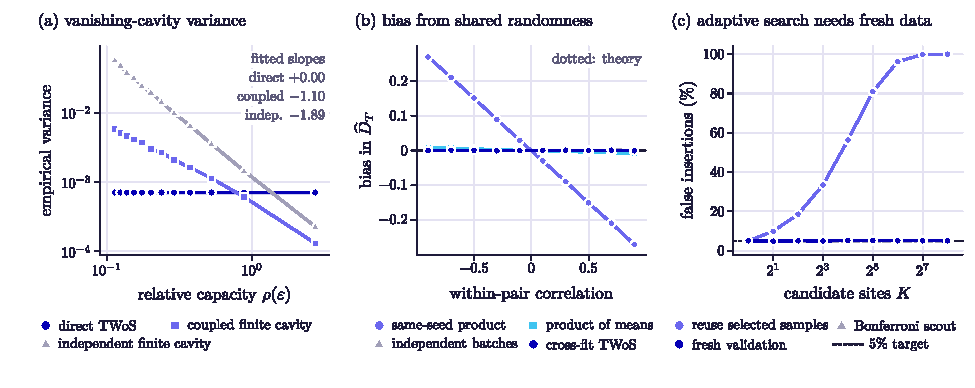
\includegraphics[width=\textwidth]{figures/controlled-experiments.pdf}
 \caption{Controlled tests of the statistical claims. (a) Direct \method{} has no insertion-radius input, so its measured variance is constant; coupled finite-cavity differencing follows the predicted $\rho^{-1}$ rare-event law, while independent solves approach the worse $\rho^{-2}$ law. Shading gives 95\% bootstrap intervals. (b) Same-seed multiplication inherits the full covariance bias and the product of sample means retains $1/N$ of it. The leave-diagonal-out estimator remains unbiased up to Monte Carlo error; independent batches are the unbiased no-reuse reference. (c) Reusing the most negative scout loses nominal coverage as the candidate count grows. Fresh validation and a simultaneous Bonferroni scout both meet the 5\% target; fresh validation controls the preselected-site test in this known-noise diagnostic.}
 \label{fig:controlled}
\end{figure}

Correlated-pair tests confirm the covariance bias predicted for same-index products. Cross-fitting and fully independent primal/adjoint batches both remove it; cross-fitting is not uniformly lower variance. The manufactured harmonic fields in \cref{fig:manufactured} test this product algebra spatially. A separate Poisson-compliance disk test has a genuine analytic topological derivative, $D_T(z)=-(1-|z|^2)^2/16$. There, independently randomized Array-RQMC batches reduce MSE by $19.9\times$ relative to ordinary Monte Carlo at equal path count, while taking longer in the measured Python implementation (\cref{fig:accelerated}). Statistical efficiency and runtime are reported separately.

The adaptive-selection test uses null candidates with known Gaussian noise. Selecting and testing with the same samples produces almost certain false acceptance among 256 sites; fresh validation and simultaneous Bonferroni bounds produce rates near the nominal $5\%$. This isolates selection error. It does not measure coverage for finite 3D insertions. The general-objective certificate also requires numerical remainder and bias bounds; the specialized cooling validator is evaluated separately below.

\subsection{Compatibility with connected refinement}

On the housing, a topological-score-weighted candidate graph initializes a connected 22-ball cavity between two internal terminals. Every trial enforces strict overlap and the same fixed-Sobol removed volume. Six Differential WoS refinement rounds propose control-point motions; fresh paired Student-$t$ tests with a Bonferroni allocation accept three steps. Independent evaluation reports a $2.086\%$ objective decrease from the graph initialization. The graph initialization itself does not measurably outperform the straight connection in this example. The channel remains sealed inside the housing, and the interval coverage relies on the paired-normal model. This experiment demonstrates compatibility between cavity initialization and existing-boundary refinement; it does not establish accessible coolant routing or a certified global topology optimum. \Cref{fig:housingchannels,fig:offsetseamsweep} report the geometry, derivative checks, and finite-offset sensitivity.

\subsection{Minimum-benefit validation on application geometry}
\label{sec:applicationvalidation}

We separately deploy the average-trace certificate in a six-attempt design
on each object. A scout-and-rescore pass fixes one finalist; fresh clipped
walks then bound its finite benefit before insertion. The validator uses
conservative triangle-box distance bounds, explicit source enclosures, and
an error budget of $0.01$ across both objects and all predeclared sampling
stages. Its probabilistic guarantee remains conditional on ideal sampling
laws and the stated input-geometry assumptions.

All twelve insertions pass the fixed absolute targets, yielding cumulative
benefit lower bounds of $5.75\times10^{-4}$ for the Bunny and
$6.21\times10^{-3}$ for the housing. Independent WoS evaluations estimate
$8.45\times10^{-4}$ and $1.020\times10^{-2}$, respectively; a separate
multigrid reference agrees on total benefits within $0.7\%$. The
average-trace bound is substantially tighter than our temperature-floor
bound on the same data (\cref{fig:applicationvalidation}). Eleven targets pass
at 1,024 walks and one at 4,096 walks, but the full four-stage diagnostic costs
$150.39$\,s and $52.17$\,s of validation time, versus $2.97$\,s and
$0.53$\,s for scouting and rescoring. This is a conservative validation
experiment, not an extension of the earlier ranking-only speed claim.
\Cref{app:applicationcertificate} gives every proof, target, timing boundary,
and numerical qualification.

\begin{figure}[t]
 \centering
 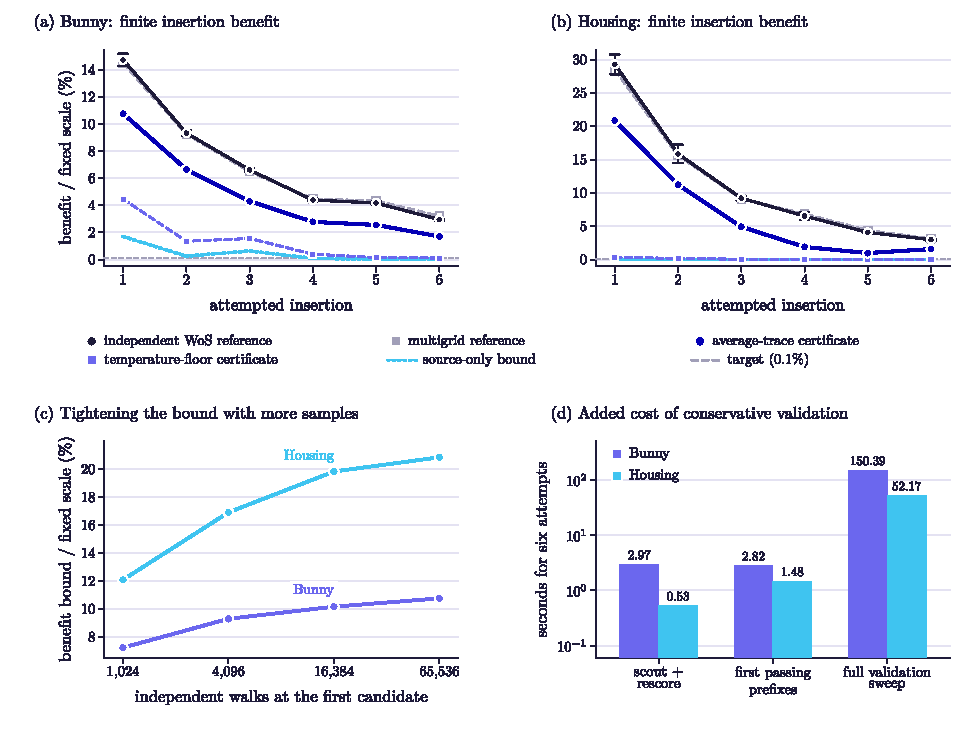
\includegraphics[width=\textwidth]{figures/application-minimum-benefit.pdf}
 \caption{\textbf{A finite benefit bound that can be evaluated before insertion.}
 (a,b) The average-trace certificate is tighter than the temperature-floor
 certificate and source-only bound on the same proposed cavities. Separate
 WoS and multigrid evaluations estimate the actual benefit; error bars show
 one spatial-block standard error for WoS. Percent axes use fixed scales
 $0.002$ (Bunny) and $0.015$ (housing), not certified baseline objectives.
 The dashed horizontal line marks the primary $0.1\%$-of-scale target.
 (c) Larger validation batches tighten the first candidate's bound.
 (d) Complete six-attempt kernel costs, with recorded first-passing prefixes
 shown separately from the full diagnostic actually executed. The bounds
 assume the stated conditional sampling laws and valid input geometry;
 numerical guard audits are reported separately.}
 \label{fig:applicationvalidation}
\end{figure}
